% Standalone rendering of every figure and table in the TMLR paper, so the
% figure and table sources in this repository can be built and checked
% without the manuscript, which is not distributed.
%
%   python paper/tmlr/build_figures.py            # full render, data/tmlr/figures.pdf
%   python paper/tmlr/build_figures.py --public   # the tracked figures.pdf
%
% Build through build_figures.py only: it writes the full render outside the
% repository and switches the citation content off for the tracked copy.
%
% Data comes from ../../data: pgfplots/tmlr/ for the figures (export stage),
% tmlr/ for the macros and the generated tables (make_macros.py and
% make_tables.py). paper/tmlr/tables/ holds the two tables that carry no
% computed value. A figure or table whose input was not built (the citation
% outputs, without the reader's own citation counts; the self-audit, without
% the manuscript) is replaced by a note saying why. Captions keep their
% \cite and \ref commands, which print as ?? here. The tikz and pgfplots setup
% matches the manuscript preamble, so the figures render as they do there.
\documentclass[10pt]{article}
\usepackage[letterpaper,margin=1in]{geometry}
\usepackage[utf8]{inputenc}
\usepackage[T1]{fontenc}
\usepackage{textcomp}
\usepackage{url}
\usepackage{booktabs}
\usepackage{caption}
\captionsetup[table]{skip=8pt}
\usepackage{amsfonts}
\usepackage{amsmath}
\usepackage{nicefrac}
\usepackage{xcolor}
\usepackage{graphicx}
\usepackage[numbers]{natbib}
\usepackage{tikz}
\usetikzlibrary{arrows.meta, positioning, shapes.geometric, fit, backgrounds}
\usepackage{pgfplots}
\usepackage{pgfplotstable}
\pgfplotsset{compat=1.18,
  every axis/.append style={
    /pgf/number format/1000 sep={},
    /pgf/number format/fixed,
  }
}
\usepgfplotslibrary{groupplots}
\DeclareUnicodeCharacter{2191}{\ensuremath{\uparrow}}
\DeclareUnicodeCharacter{2193}{\ensuremath{\downarrow}}

% The manuscript marks revised text with these for its review build; here
% they print their argument unchanged, as in the published paper.
\newcommand{\rev}[1]{#1}
\newcommand{\revtwo}[1]{#1}
\newcommand{\revthree}[1]{#1}
\newcommand{\revfour}[1]{#1}

\newcommand{\aadata}{../../data}
\newcommand{\aanote}[1]{\begin{center}\fbox{\parbox{0.9\linewidth}{\small #1}}\end{center}}
% \aainput{file}{what}{why}: input file, or a note when it was not built.
\newcommand{\aainput}[3]{\IfFileExists{#1}{\input{#1}}{\aanote{#2 not rendered: #3}}}
\newcommand{\aamacros}[1]{\IfFileExists{\aadata/tmlr/#1}{\input{\aadata/tmlr/#1}}{}}
\aamacros{generated_round2.tex}
\aamacros{generated_round3.tex}
\aamacros{generated_round4.tex}
\newcommand{\aatable}[2]{\aainput{\aadata/tmlr/tables/#1}{Table \texttt{\detokenize{#1}}}{#2}}
\newcommand{\nocit}{the citation outputs were not built (the citation counts are
  not distributed; see README, Citations)}
\newcommand{\nopipe}{its input was not built; see \texttt{data/incomplete.json}
  and \texttt{data/tmlr/}}
% build_figures.py defines \aacitationsabsent when the local citation counts
% are absent, so an output left from an earlier run is not rendered.
\newcommand{\aacitations}[2]{\ifdefined\aacitationsabsent\aanote{#2 not rendered:
  \nocit}\else#1\fi}

\title{abstract-audit: TMLR figure and table sources}
\author{}
\date{}

\begin{document}
\maketitle

\section*{Main text}

\begin{table}[t]
  \centering
  \small
  \begin{tabular}{p{0.20\textwidth}p{0.30\textwidth}p{0.12\textwidth}p{0.26\textwidth}}
    \toprule
    Family & What it measures & Section & Direction over time \\
    \midrule
    Classical readability, 15 formulas
      & Surface difficulty of the prose, from sentence length and word length
      & \ref{sec:readability-classical}
      & Harder to read at every venue \\
    \addlinespace
    Hohmann writing style suite, \revfour{extended to 12 metrics}
      & Syntactic structure, including parse depth, passive rate and noun
        phrase density
      & \ref{sec:hohmann}
      & Largely parallel to the non-ML control \\
    \addlinespace
    Sensational language rate\revfour{, part of the style suite}
      & Rhetorical stance, counted as promotional words per 100 words
      & \ref{sec:sensational}
      & Rising at every venue \\
    \addlinespace
    Acronym density and reuse
      & Vocabulary a reader must already hold, and how often each term recurs
      & \ref{sec:acronyms}
      & Denser, with most terms rarely reused \\
    \addlinespace
    LLM as judge, 6 models
      & What an automated reviewer reports about readability
      & \ref{sec:llm-judge}
      & Rising after 2022 at NeurIPS and ICML, against the classical scores \\
    \addlinespace
    Citation counts
      & What the field rewarded, within venue-year cohorts
      & \ref{sec:citations}
      & More readable papers cited slightly more \\
    \bottomrule
  \end{tabular}
\caption{\revthree{The five metric families, what each one measures, and the
  direction it moves at NeurIPS, ICLR and ICML.}}
  \label{tab:families}
\end{table}

% Flesch Reading Ease on NeurIPS, arXiv ML, arXiv non-ML, and PubMed.
% Data: ../../data/tmlr/pgfplots/readability_flesch_ease.csv
% Higher values = easier reading.

\begin{figure}[h]
\centering
\begin{tikzpicture}
\begin{axis}[
    width=0.88\linewidth, height=5cm,
    xlabel={Year},
    ylabel={Flesch Reading Ease (\textuparrow\ easier)},
    xtick distance=8,
    x tick label style={rotate=45, anchor=east, font=\tiny,
                        /pgf/number format/1000 sep={}},
    ytick align=inside,
    legend columns=3,
    legend style={draw=none, fill=none, font=\scriptsize,
                  cells={anchor=west}, column sep=8pt,
                  at={(0.5,-0.28)}, anchor=north},
    tick label style={font=\tiny},
    label style={font=\small},
    enlarge x limits=0.02,
  ]
  \addplot[color={rgb,255:red,44;green,160;blue,44}, dashdotted, very thick]
    table[x=year, y=neurips, col sep=comma]
    {../../data/tmlr/pgfplots/readability_flesch_ease.csv};
  \addlegendentry{NeurIPS}
  \addplot[color={rgb,255:red,31;green,119;blue,180}, densely dashed, very thick]
    table[x=year, y=iclr, col sep=comma]
    {../../data/tmlr/pgfplots/readability_flesch_ease.csv};
  \addlegendentry{ICLR}
  \addplot[color={rgb,255:red,255;green,127;blue,14}, densely dotted, very thick]
    table[x=year, y=icml, col sep=comma]
    {../../data/tmlr/pgfplots/readability_flesch_ease.csv};
  \addlegendentry{ICML}
  \addplot[color={rgb,255:red,148;green,103;blue,189}, solid, very thick]
    table[x=year, y=arxiv_ml, col sep=comma]
    {../../data/tmlr/pgfplots/readability_flesch_ease.csv};
  \addlegendentry{arXiv ML}
  \addplot[color={rgb,255:red,140;green,86;blue,75}, dotted, thick]
    table[x=year, y=arxiv_nonml, col sep=comma]
    {../../data/tmlr/pgfplots/readability_flesch_ease.csv};
  \addlegendentry{arXiv non-ML}
  \addplot[color={rgb,255:red,214;green,39;blue,40}, dashed, thick]
    table[x=year, y=pubmed, col sep=comma]
    {../../data/tmlr/pgfplots/readability_flesch_ease.csv};
  \addlegendentry{PubMed}
  % Marker for the arrival of LLM assisted writing (late 2022)
  \draw[black, dashed, semithick] (axis cs:2022,-5) -- (axis cs:2022,50);
  \node[font=\tiny, anchor=east, align=right]
    at (axis cs:2021.7,32) {\revfour{LLM assisted}\\\revfour{writing (2022)}};
\end{axis}
\end{tikzpicture}
\caption{\textbf{Flesch Reading Ease across all six corpora
  (NeurIPS, ICLR, ICML, arXiv ML, arXiv non-ML, and PubMed),
  1987--2026.}
  Higher values indicate easier reading (\textuparrow).
  \rev{The three conferences and arXiv ML all decline, and by 2025 each
  sits below both the arXiv non-ML and the PubMed baseline.}}
\label{fig:readability-flesch}
\end{figure}

% Total sensational language per 100 abstract words.
% Data: ../../data/pgfplots/tmlr/sensational_total.csv

\begin{figure}[h]
\centering
\begin{tikzpicture}
\begin{axis}[
    width=0.88\linewidth, height=5cm,
    xlabel={Year},
    ylabel={Total sensational words per 100},
    xtick distance=8,
    x tick label style={rotate=45, anchor=east, font=\tiny,
                        /pgf/number format/1000 sep={}},
    ytick align=inside,
    legend columns=3,
    legend style={draw=none, fill=none, font=\scriptsize,
                  cells={anchor=west}, column sep=8pt,
                  at={(0.5,-0.28)}, anchor=north},
    tick label style={font=\tiny},
    label style={font=\small},
    enlarge x limits=0.02,
    ymin=0,
  ]
  \addplot[color={rgb,255:red,44;green,160;blue,44}, dashdotted, very thick]
    table[x=year, y=neurips, col sep=comma]
    {../../data/pgfplots/tmlr/sensational_total.csv};
  \addlegendentry{NeurIPS}
  \addplot[color={rgb,255:red,31;green,119;blue,180}, densely dashed, very thick]
    table[x=year, y=iclr, col sep=comma]
    {../../data/pgfplots/tmlr/sensational_total.csv};
  \addlegendentry{ICLR}
  \addplot[color={rgb,255:red,255;green,127;blue,14}, densely dotted, very thick]
    table[x=year, y=icml, col sep=comma]
    {../../data/pgfplots/tmlr/sensational_total.csv};
  \addlegendentry{ICML}
  \addplot[color={rgb,255:red,148;green,103;blue,189}, solid, very thick]
    table[x=year, y=arxiv_ml, col sep=comma]
    {../../data/pgfplots/tmlr/sensational_total.csv};
  \addlegendentry{arXiv ML}
  \addplot[color={rgb,255:red,140;green,86;blue,75}, dotted, thick]
    table[x=year, y=arxiv_nonml, col sep=comma]
    {../../data/pgfplots/tmlr/sensational_total.csv};
  \addlegendentry{arXiv non-ML}
  \addplot[color={rgb,255:red,214;green,39;blue,40}, dashed, thick]
    table[x=year, y=pubmed, col sep=comma]
    {../../data/pgfplots/tmlr/sensational_total.csv};
  \addlegendentry{PubMed}
  % ChatGPT launch marker (line only; the text label appears
  % only in fig:readability-flesch, the first chronological figure).
  \draw[black, dashed, semithick] (axis cs:2022,0) -- (axis cs:2022,30);
\end{axis}
\end{tikzpicture}
\caption{\textbf{Total sensational language per 100 abstract words,
  1987--\revfour{2026}.}
  \rev{The rate rises across all three conferences and arXiv ML. The
  arXiv non-ML baseline rises far
  more slowly, and the divergence between ML and non-ML venues
  accelerates after 2022.}
  The \revfour{breakdown by category} appears in
  Appendix~\ref{app:figures}.}
\label{fig:sensational-total}
\end{figure}

% LLM-as-judge: model-averaged z-scores per venue, one curve per prompt.
% Each curve is the mean of all 6 model z-scores for that prompt, standardized
% to each model's own baseline through 2022 within that venue.
% Data: ../../data/pgfplots/llm_scores_model_avg[_{venue}]_{prompt}.csv

% One panel's three prompt curves + zero line + 2022 marker.
% #1 = file suffix: "" (NeurIPS), "_iclr", "_icml"
\providecommand{\llmpanel}[1]{%
  \addplot[color={rgb,255:red,44;green,160;blue,44}, solid, very thick]
    table[x=year, y=avg_z, col sep=comma]{../../data/pgfplots/llm_scores_model_avg#1_simple.csv};
  \addplot[color={rgb,255:red,148;green,103;blue,189}, dashed, very thick]
    table[x=year, y=avg_z, col sep=comma]{../../data/pgfplots/llm_scores_model_avg#1_ascb.csv};
  \addplot[color={rgb,255:red,214;green,39;blue,40}, dashdotted, very thick]
    table[x=year, y=avg_z, col sep=comma]{../../data/pgfplots/llm_scores_model_avg#1_own_reasoning.csv};
  \draw[black, dotted, thin] (axis cs:1900,0) -- (axis cs:2100,0);
  \draw[black, dashed, semithick] (axis cs:2022,-2) -- (axis cs:2022,5.5);
}

\begin{figure}[h]
\centering
\begin{tikzpicture}
\begin{groupplot}[
    group style={group size=3 by 1, horizontal sep=10mm},
    width=0.30\linewidth, height=4.3cm,
    ymin=-2, ymax=5.5,
    xtick distance=8,
    x tick label style={rotate=45, anchor=east, font=\tiny,
                        /pgf/number format/1000 sep={}},
    y tick label style={font=\tiny},
    ytick align=inside,
    enlarge x limits=0.03,
    title style={font=\small, yshift=-1mm},
  ]
  \nextgroupplot[title={NeurIPS}, ylabel={Model-averaged readability (z)},
    ylabel style={font=\tiny},
    legend to name=llmlegend, legend columns=3,
    legend style={draw=none, fill=none, font=\scriptsize,
                  cells={anchor=west}, column sep=8pt}]
  \addplot[color={rgb,255:red,44;green,160;blue,44}, solid, very thick]
    table[x=year, y=avg_z, col sep=comma]{../../data/pgfplots/llm_scores_model_avg_simple.csv};
  \addlegendentry{Simple}
  \addplot[color={rgb,255:red,148;green,103;blue,189}, dashed, very thick]
    table[x=year, y=avg_z, col sep=comma]{../../data/pgfplots/llm_scores_model_avg_ascb.csv};
  \addlegendentry{ASCB}
  \addplot[color={rgb,255:red,214;green,39;blue,40}, dashdotted, very thick]
    table[x=year, y=avg_z, col sep=comma]{../../data/pgfplots/llm_scores_model_avg_own_reasoning.csv};
  \addlegendentry{Own reasoning}
  \draw[black, dotted, thin] (axis cs:1900,0) -- (axis cs:2100,0);
  \draw[black, dashed, semithick] (axis cs:2022,-2) -- (axis cs:2022,5.5);

  \nextgroupplot[title={ICLR}]
  \llmpanel{_iclr}

  \nextgroupplot[title={ICML}]
  \llmpanel{_icml}
\end{groupplot}
\end{tikzpicture}

\vspace{1mm}
\pgfplotslegendfromname{llmlegend}

\caption{\textbf{LLM as judge readability across the three conferences.}
  Each curve is the mean z-score across all six open-weight models for one
  prompt variant, standardized to each model's own \revfour{baseline through 2022} within
  that venue. NeurIPS and
  ICML show the same pattern. \revfour{Scores rise sharply after 2022,
  by roughly three to five standard deviations}, directly contradicting
  the classical readability decline in Figure~\ref{fig:readability-flesch}.
  \rev{ICLR shows no comparable rise, and its post-2022 movement does not settle
  into a consistent trend across the three prompts, so we draw no conclusion
  from that series and leave it to further investigation.}}
\label{fig:llm-judge}
\end{figure}

\clearpage
% Acronym density -- title (left) and abstract (right).
% Data: ../../data/pgfplots/tmlr/acronyms_title.csv, acronyms_abstract.csv

\begin{figure}[h]
\centering
\pgfplotsset{
  acro style/.style={
    height=5cm, width=0.47\linewidth,
    xlabel={Year}, ylabel={Acronyms per 100 words},
    xtick distance=8, x tick label style={rotate=45, anchor=east, font=\tiny,
                                          /pgf/number format/1000 sep={}},
    ytick align=inside, ymin=0,
    tick label style={font=\tiny}, label style={font=\small},
    enlarge x limits=0.02,
  }
}
% -- title density: legend collected here ----------------------------------
\begin{tikzpicture}
\begin{axis}[acro style,
  title={\small Titles~[\textdownarrow\ better]},
  legend to name=acrolegend,
  legend columns=4,
  legend style={draw=none, fill=none, font=\scriptsize,
                cells={anchor=west}, column sep=6pt},
]
  \addplot[color={rgb,255:red,44;green,160;blue,44}, dashdotted, very thick]
    table[x=year, y=neurips, col sep=comma] {../../data/pgfplots/tmlr/acronyms_title.csv};
  \addlegendentry{NeurIPS}
  \addplot[color={rgb,255:red,31;green,119;blue,180}, densely dashed, very thick]
    table[x=year, y=iclr, col sep=comma] {../../data/pgfplots/tmlr/acronyms_title.csv};
  \addlegendentry{ICLR}
  \addplot[color={rgb,255:red,255;green,127;blue,14}, densely dotted, very thick]
    table[x=year, y=icml, col sep=comma] {../../data/pgfplots/tmlr/acronyms_title.csv};
  \addlegendentry{ICML}
  \addplot[color={rgb,255:red,148;green,103;blue,189}, solid, very thick]
    table[x=year, y=arxiv_ml, col sep=comma] {../../data/pgfplots/tmlr/acronyms_title.csv};
  \addlegendentry{arXiv ML}
  \addplot[color={rgb,255:red,140;green,86;blue,75}, dotted, thick]
    table[x=year, y=arxiv_nonml, col sep=comma] {../../data/pgfplots/tmlr/acronyms_title.csv};
  \addlegendentry{arXiv non-ML}
  \addplot[color={rgb,255:red,214;green,39;blue,40}, dashed, thick]
    table[x=year, y=pubmed, col sep=comma] {../../data/pgfplots/tmlr/acronyms_title.csv};
  \addlegendentry{PubMed}
  \addplot[black, dashed, semithick, domain=1987:2025] {2.40};
  \addlegendentry{Barnett 2020 titles (2.40)}
  \draw[black, dashed, semithick] (axis cs:2022,0) -- (axis cs:2022,100);
\end{axis}
\end{tikzpicture}%
\hfill
% -- abstract density ------------------------------------------------------
\begin{tikzpicture}
\begin{axis}[acro style, title={\small Abstracts~[\textdownarrow\ better]}]
  \addplot[color={rgb,255:red,44;green,160;blue,44}, dashdotted, very thick]
    table[x=year, y=neurips, col sep=comma] {../../data/pgfplots/tmlr/acronyms_abstract.csv};
  \addplot[color={rgb,255:red,31;green,119;blue,180}, densely dashed, very thick]
    table[x=year, y=iclr, col sep=comma] {../../data/pgfplots/tmlr/acronyms_abstract.csv};
  \addplot[color={rgb,255:red,255;green,127;blue,14}, densely dotted, very thick]
    table[x=year, y=icml, col sep=comma] {../../data/pgfplots/tmlr/acronyms_abstract.csv};
  \addplot[color={rgb,255:red,148;green,103;blue,189}, solid, very thick]
    table[x=year, y=arxiv_ml, col sep=comma] {../../data/pgfplots/tmlr/acronyms_abstract.csv};
  \addplot[color={rgb,255:red,140;green,86;blue,75}, dotted, thick]
    table[x=year, y=arxiv_nonml, col sep=comma] {../../data/pgfplots/tmlr/acronyms_abstract.csv};
  \addplot[color={rgb,255:red,214;green,39;blue,40}, dashed, thick]
    table[x=year, y=pubmed, col sep=comma] {../../data/pgfplots/tmlr/acronyms_abstract.csv};
  \addplot[black, dashed, semithick, domain=1987:2025] {4.10};
  \draw[black, dashed, semithick] (axis cs:2022,0) -- (axis cs:2022,100);
\end{axis}
\end{tikzpicture}

\vspace{2mm}
\pgfplotslegendfromname{acrolegend}

\caption{\textbf{Acronym density in titles (left) and abstracts
  (right), 1987 to \revfour{2026}.}
  \rev{\citet{barnett2020growth} report acronym density for titles and
  for abstracts separately, and their 2019 \revfour{biomedical} values
  differ between the two. The dashed black horizontal line marks
  the applicable one in each panel, 2.40 per 100 words for titles
  and 4.10 for abstracts. ML title density has risen above the
  \revfour{biomedical} title value, while ML abstract density remains
  below the \revfour{biomedical} abstract value.}}
\label{fig:acronyms}
\end{figure}

\aacitations{\aatable{topics.tex}{\nocit}}{Table topics.tex}
\clearpage

\section*{Appendix}

\begin{figure}[h]
  \centering
  \resizebox{\linewidth}{!}{%
  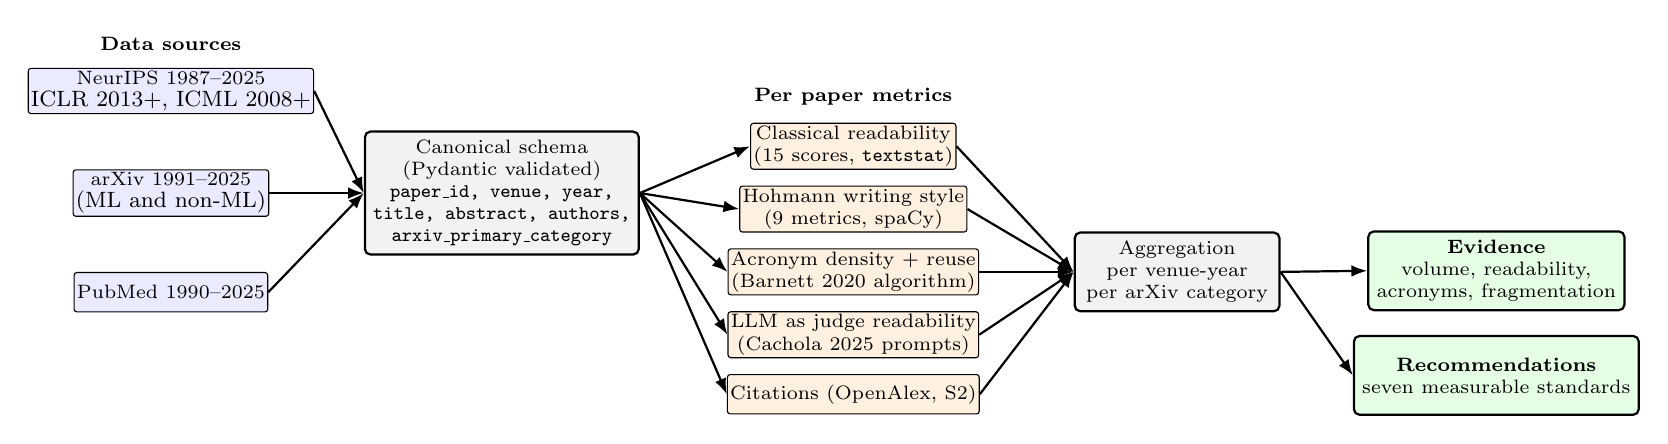
\begin{tikzpicture}[
      node distance=7mm and 9mm,
      font=\scriptsize,
      every node/.style={align=center},
      source/.style={draw, rounded corners=1pt, fill=blue!8,
                     minimum width=18mm, minimum height=5mm, inner sep=1pt},
      stage/.style={draw, thick, rounded corners=2pt, fill=gray!10,
                    minimum width=26mm, minimum height=10mm, inner sep=3pt},
      metric/.style={draw, rounded corners=1pt, fill=orange!12,
                     minimum width=26mm, minimum height=5mm, inner sep=1pt},
      output/.style={draw, thick, rounded corners=2pt, fill=green!10,
                     minimum width=30mm, minimum height=10mm, inner sep=3pt},
      flow/.style={-{Latex[length=2mm]}, thick},
    ]
    % Column 1: sources.
    \node[source] (s1) {NeurIPS 1987--2025 \\ {\footnotesize ICLR 2013+, ICML 2008+}};
    \node[source, below=of s1] (s2) {arXiv 1991--2025 \\ {\footnotesize (ML and non-ML)}};
    \node[source, below=of s2] (s3) {PubMed 1990--2025};
    \node[above=1mm of s1, font=\scriptsize\bfseries] {Data sources};

    % Column 2: canonical schema.
    \node[stage, right=12mm of s2.east] (schema)
      {Canonical schema \\ (Pydantic validated) \\
       \texttt{paper\_id, venue, year,} \\
       \texttt{title, abstract, authors,} \\
       \texttt{arxiv\_primary\_category}};

    % Column 3: per paper metrics.
    \node[metric, right=14mm of schema.north east, yshift=-2mm] (m1)
      {Classical readability \\ (15 scores, \texttt{textstat})};
    \node[metric, below=2mm of m1] (m2)
      {Hohmann writing style \\ (9 metrics, spaCy)};
    \node[metric, below=2mm of m2] (m3)
      {Acronym density + reuse \\ (Barnett 2020 algorithm)};
    \node[metric, below=2mm of m3] (m4)
      {LLM as judge readability \\ (Cachola 2025 prompts)};
    \node[metric, below=2mm of m4] (m5)
      {Citations (OpenAlex, S2)};
    \node[above=1mm of m1, font=\scriptsize\bfseries] {Per paper metrics};

    % Column 4: aggregation.
    \node[stage, right=12mm of m3.east] (agg)
      {Aggregation \\ per venue-year \\ per arXiv category};

    % Column 5: outputs.
    \node[output, right=11mm of agg.north east, yshift=-5mm] (ev)
      {\textbf{Evidence} \\ volume, readability, \\ acronyms, fragmentation};
    \node[output, below=3mm of ev] (pol)
      {\textbf{Recommendations} \\ seven measurable standards};

    % Flow arrows: sources to schema.
    \foreach \src in {s1, s2, s3}
      \draw[flow] (\src.east) -- (schema.west);

    % Schema to metrics.
    \foreach \met in {m1, m2, m3, m4, m5}
      \draw[flow] (schema.east) -- (\met.west);

    % Metrics to aggregation.
    \foreach \met in {m1, m2, m3, m4, m5}
      \draw[flow] (\met.east) -- (agg.west);

    % Aggregation to outputs.
    \draw[flow] (agg.east) -- (ev.west);
    \draw[flow] (agg.east) -- (pol.west);
  \end{tikzpicture}%
  }
  \caption{\textbf{End to end workflow.} Three data sources feed a
  canonical Pydantic-validated schema. Five per-paper metric
  families are computed \revfour{on abstracts, and acronym density
  also on titles,} then
  aggregated per venue-year and per arXiv primary category.
  The outputs feed the empirical evidence
  (Sections~\ref{sec:readability} through~\ref{sec:volume}) and
  the recommendations
  (Section~\ref{sec:policy}). Pipeline details appear in
  Appendix~\ref{app:workflow}.}
  \label{fig:workflow}
\end{figure}

\aatable{corpus.tex}{\nopipe}
\aatable{normalisation_rules.tex}{\nopipe}
\aatable{normalisation.tex}{\nopipe}
\clearpage
\aatable{prompts.tex}{\nopipe}
\clearpage
\aacitations{\aatable{topic_controls.tex}{\nocit}}{Table topic\_controls.tex}
\aatable{topic_trends.tex}{\nopipe}
\aatable{topic_decomposition.tex}{\nopipe}
\clearpage
\aatable{acronym_reuse_freq.tex}{\nopipe}
\aatable{acronym_concentration.tex}{\nopipe}
\aacitations{\aatable{citation_readability_top_bottom_combined.tex}{\nocit}}{Table
  citation\_readability\_top\_bottom\_combined.tex}
\aacitations{\aatable{citation_llm_top_bottom_combined.tex}{\nocit}}{Table
  citation\_llm\_top\_bottom\_combined.tex}
\clearpage
\aacitations{\IfFileExists{\aadata/pgfplots/tmlr/references_per_year.csv}{% Mean bibliography entries per paper, NeurIPS / ICLR / ICML.
% Data: ../../data/pgfplots/tmlr/references_per_year.csv
% Papers with no Semantic Scholar reference list are excluded rather than
% counted as zero; see src/citations/references.py.

\begin{figure}[h]
\centering
\begin{tikzpicture}
\begin{axis}[
    width=0.85\linewidth, height=5cm,
    xlabel={Year}, ylabel={Bibliography entries per paper},
    xtick distance=8,
    x tick label style={rotate=45, anchor=east, font=\tiny,
                        /pgf/number format/1000 sep={}},
    ytick align=inside,
    tick label style={font=\tiny},
    label style={font=\small},
    enlarge x limits=0.02,
    legend style={font=\tiny, at={(0.02,0.98)}, anchor=north west,
                  draw=none, fill opacity=0.7, text opacity=1},
    legend cell align=left,
  ]
  \addplot[color={rgb,255:red,44;green,160;blue,44}, dashdotted, very thick]
    table[x=year, y=neurips, col sep=comma]
    {../../data/pgfplots/tmlr/references_per_year.csv};
  \addlegendentry{NeurIPS}
  \addplot[color={rgb,255:red,31;green,119;blue,180}, densely dashed, very thick]
    table[x=year, y=iclr, col sep=comma]
    {../../data/pgfplots/tmlr/references_per_year.csv};
  \addlegendentry{ICLR}
  \addplot[color={rgb,255:red,255;green,127;blue,14}, densely dotted, very thick]
    table[x=year, y=icml, col sep=comma]
    {../../data/pgfplots/tmlr/references_per_year.csv};
  \addlegendentry{ICML}
  \draw[black, dashed, semithick] (axis cs:2022,0) -- (axis cs:2022,100);
\end{axis}
\end{tikzpicture}
\caption{\textbf{Mean bibliography length per paper at the three
  conferences.}
  \rev{Reference list length grows steadily at every venue and then
  levels off. NeurIPS rises from roughly 11 entries per paper in
  1987 to a peak of 62.9 in 2022 and holds between 59 and 61
  through 2025. ICLR, from 2013, and ICML, from 2008, converge on
  the same band, reaching 57 to 61 entries by 2025. Papers for which
  Semantic Scholar holds no reference list are excluded, and
  coverage of the most recent year is lower than of earlier years
  (73 percent of NeurIPS 2025, against 97 percent for 2022).}}
\label{fig:app-references}
\end{figure}
}{\aanote{Figure
  fig\_app\_references not rendered: \nocit}}}{Figure fig\_app\_references}
% Papers per year on a log scale.
% Data: ../../data/pgfplots/papers_per_year.csv

\begin{figure}[h]
\centering
\begin{tikzpicture}
\begin{axis}[
    width=0.88\linewidth, height=5cm,
    xlabel={Year}, ylabel={Papers per year (log scale)},
    ymode=log,
    xtick distance=8,
    x tick label style={rotate=45, anchor=east, font=\tiny,
                        /pgf/number format/1000 sep={}},
    ytick align=inside,
    legend columns=3,
    legend style={draw=none, fill=none, font=\scriptsize,
                  cells={anchor=west}, column sep=8pt,
                  at={(0.5,-0.28)}, anchor=north},
    tick label style={font=\tiny}, label style={font=\small},
    enlarge x limits=0.02,
  ]
  \addplot[color={rgb,255:red,44;green,160;blue,44}, dashdotted, very thick]
    table[x=year, y=neurips, col sep=comma] {../../data/pgfplots/papers_per_year.csv};
  \addlegendentry{NeurIPS}
  \addplot[color={rgb,255:red,31;green,119;blue,180}, densely dashed, very thick]
    table[x=year, y=iclr, col sep=comma] {../../data/pgfplots/papers_per_year.csv};
  \addlegendentry{ICLR}
  \addplot[color={rgb,255:red,255;green,127;blue,14}, densely dotted, very thick]
    table[x=year, y=icml, col sep=comma] {../../data/pgfplots/papers_per_year.csv};
  \addlegendentry{ICML}
  \addplot[color={rgb,255:red,148;green,103;blue,189}, solid, very thick]
    table[x=year, y=arxiv_ml, col sep=comma] {../../data/pgfplots/papers_per_year.csv};
  \addlegendentry{arXiv ML}
  \addplot[color={rgb,255:red,140;green,86;blue,75}, dotted, thick]
    table[x=year, y=arxiv_nonml, col sep=comma] {../../data/pgfplots/papers_per_year.csv};
  \addlegendentry{arXiv non-ML}
  \addplot[color={rgb,255:red,214;green,39;blue,40}, dashed, thick]
    table[x=year, y=pubmed, col sep=comma] {../../data/pgfplots/papers_per_year.csv};
  \addlegendentry{PubMed}
  \draw[black, dashed, semithick] (axis cs:2022,1) -- (axis cs:2022,1e8);
\end{axis}
\end{tikzpicture}

\vspace{2mm}

\caption{\textbf{Papers per year, 1987 to \revfour{2026}.}
  arXiv ML submissions grew by roughly four orders of magnitude
  between 1993 and 2025. NeurIPS grew by a factor of roughly 65
  between 1987 and 2025, from fewer than 100 accepted papers to
  approximately 5,800. PubMed and arXiv non-ML show
  sustained but slower growth over the same period. The volume
  increase is the structural backdrop against which the
  readability and acronym trends in
  Sections~\ref{sec:readability} and~\ref{sec:acronyms} must
  be interpreted.}
\label{fig:papers}
\end{figure}

\begin{table}[h]
  \centering
  \begin{tabular}{ll}
    \toprule
    Metric & Primary sources \\
    \midrule
    Sentence length      & \citet{britton1982sentence, jeong2021readability} \\
    Sign posting         & \citet{lindsay2011scientific, montgomery2003chicago} \\
    Hedging              & \citet{montgomery2003chicago, pinker2014sense, sword2012stylish} \\
    Noun chunks          & \citet{lindsay2011scientific, montgomery2003chicago, pinker2014sense} \\
    Active narration     & \citet{hillier2016narrative, pinker2014sense, sword2012stylish} \\
    Verbs                & \citet{hillier2016narrative, ryba2019verbs} \\
    Nouns                & \citet{crossley2017nouns} \\
    Numbers              & \citet{stremersch2007numbers} \\
    Sensational language & \citet{millar2022sensational} \\
    \bottomrule
  \end{tabular}
  \caption{Writing style metrics audited per paper, with the
  original sources cited by \citet{hohmann2025evolution}.}
  \label{tab:nine}
\end{table}

\clearpage
% Classical readability: appendix, split into two 3-column figures
% to fit within the NeurIPS text width.
% Data: ../../data/pgfplots/readability_<metric>.csv

\providecommand{\readpanel}[3]{%
  \nextgroupplot[title={\tiny #1~[#3]},
                 title style={font=\tiny, yshift=-1.5mm}]
  \addplot[color={rgb,255:red,44;green,160;blue,44}, dashdotted, very thick]
    table[x=year, y=neurips, col sep=comma]{../../data/pgfplots/#2.csv};
  \addplot[color={rgb,255:red,31;green,119;blue,180}, densely dashed, very thick]
    table[x=year, y=iclr, col sep=comma]{../../data/pgfplots/#2.csv};
  \addplot[color={rgb,255:red,255;green,127;blue,14}, densely dotted, very thick]
    table[x=year, y=icml, col sep=comma]{../../data/pgfplots/#2.csv};
  \addplot[color={rgb,255:red,148;green,103;blue,189}, solid, thick]
    table[x=year, y=arxiv_ml, col sep=comma]{../../data/pgfplots/#2.csv};
  \addplot[color={rgb,255:red,140;green,86;blue,75}, dotted, thick]
    table[x=year, y=arxiv_nonml, col sep=comma]{../../data/pgfplots/#2.csv};
  \addplot[color={rgb,255:red,214;green,39;blue,40}, dashed, thick]
    table[x=year, y=pubmed, col sep=comma]{../../data/pgfplots/#2.csv};
  \draw[black, dashed, semithick]
    ({axis cs:2022,0} |- {rel axis cs:0,0})
    -- ({axis cs:2022,0} |- {rel axis cs:0,1});
}

% ── Figure A: 8 readability metrics, 3 by 3 layout (1 blank slot) ────────────
\begin{figure}[htbp]
\centering
\begin{tikzpicture}
\begin{groupplot}[
    group style={
      group size=3 by 3,
      horizontal sep=8mm,
      vertical sep=12mm,
    },
    width=40mm, height=2.4cm,
    scale only axis,
    xlabel={}, ylabel={},
    xtick distance=12,
    x tick label style={rotate=55, anchor=east, font=\tiny,
                        /pgf/number format/1000 sep={}},
    y tick label style={font=\tiny},
    ytick align=inside,
    enlarge x limits=0.02,
    tick label style={font=\tiny},
  ]
  % First panel: legend collected here
  \nextgroupplot[
    title={\tiny Flesch Ease~[\textuparrow]},
    title style={font=\tiny, yshift=-1.5mm},
    legend to name=readlegend,
    legend columns=3,
    legend style={draw=none, fill=none, font=\scriptsize,
                  cells={anchor=west}, column sep=8pt},
  ]
  \addplot[color={rgb,255:red,44;green,160;blue,44}, dashdotted, very thick]
    table[x=year, y=neurips, col sep=comma]{../../data/pgfplots/readability_flesch_ease.csv};
  \addlegendentry{NeurIPS}
  \addplot[color={rgb,255:red,31;green,119;blue,180}, densely dashed, very thick]
    table[x=year, y=iclr, col sep=comma]{../../data/pgfplots/readability_flesch_ease.csv};
  \addlegendentry{ICLR}
  \addplot[color={rgb,255:red,255;green,127;blue,14}, densely dotted, very thick]
    table[x=year, y=icml, col sep=comma]{../../data/pgfplots/readability_flesch_ease.csv};
  \addlegendentry{ICML}
  \addplot[color={rgb,255:red,148;green,103;blue,189}, solid, thick]
    table[x=year, y=arxiv_ml, col sep=comma]{../../data/pgfplots/readability_flesch_ease.csv};
  \addlegendentry{arXiv ML}
  \addplot[color={rgb,255:red,140;green,86;blue,75}, dotted, thick]
    table[x=year, y=arxiv_nonml, col sep=comma]{../../data/pgfplots/readability_flesch_ease.csv};
  \addlegendentry{arXiv non-ML}
  \addplot[color={rgb,255:red,214;green,39;blue,40}, dashed, thick]
    table[x=year, y=pubmed, col sep=comma]{../../data/pgfplots/readability_flesch_ease.csv};
  \addlegendentry{PubMed}
  \draw[black, dashed, semithick]
    ({axis cs:2022,0} |- {rel axis cs:0,0})
    -- ({axis cs:2022,0} |- {rel axis cs:0,1});
  % Remaining 7 panels of part A
  \readpanel{Flesch--Kincaid}{readability_flesch_kincaid}{\textdownarrow}
  \readpanel{Gunning Fog}{readability_gunning_fog}{\textdownarrow}
  \readpanel{SMOG}{readability_smog}{\textdownarrow}
  \readpanel{Dale--Chall}{readability_dale_chall}{\textdownarrow}
  \readpanel{Spache}{readability_spache}{\textdownarrow}
  \readpanel{Coleman--Liau}{readability_coleman_liau}{\textdownarrow}
  \readpanel{ARI}{readability_ari}{\textdownarrow}
  % 9th slot blank for layout
  \nextgroupplot[hide axis, scale only axis, width=40mm, height=2.4cm]
\end{groupplot}
\end{tikzpicture}

\vspace{2mm}
\pgfplotslegendfromname{readlegend}

\caption{\textbf{Classical readability metrics, part A: Flesch
  family and grade-level formulas, 1987--\revfour{2026}.}
  Arrows indicate the direction of easier reading
  (\textuparrow\ = higher is better, \textdownarrow\ = lower is
  better). Every grade-level metric rises on NeurIPS and arXiv
  ML after 2015 and accelerates after 2020. Flesch Reading Ease
  drops correspondingly. Vertical dashed lines mark the
  late-2022 availability of instruction-tuned writing
  assistants. Part B with the remaining seven metrics appears in
  Figure~\ref{fig:app-readability-b}.}
\label{fig:app-readability}
\end{figure}

% ── Figure B: 7 readability metrics, 3 by 3 layout (2 blank slots) ───────────
\begin{figure}[htbp]
\centering
\begin{tikzpicture}
\begin{groupplot}[
    group style={
      group size=3 by 3,
      horizontal sep=8mm,
      vertical sep=12mm,
    },
    width=40mm, height=2.4cm,
    scale only axis,
    xlabel={}, ylabel={},
    xtick distance=12,
    x tick label style={rotate=55, anchor=east, font=\tiny,
                        /pgf/number format/1000 sep={}},
    y tick label style={font=\tiny},
    ytick align=inside,
    enlarge x limits=0.02,
    tick label style={font=\tiny},
  ]
  \readpanel{Linsear Write}{readability_linsear_write}{\textdownarrow}
  \readpanel{LIX}{readability_lix}{\textdownarrow}
  \readpanel{RIX}{readability_rix}{\textdownarrow}
  \readpanel{FORCAST}{readability_forcast}{\textdownarrow}
  \readpanel{Pwr--Smnr--Kearl}{readability_powers_sumner_kearl}{\textdownarrow}
  \readpanel{Sentence length}{readability_avg_sentence_length}{\textdownarrow}
  \readpanel{Syllables/word}{readability_avg_syllables_per_word}{\textdownarrow}
  % Two blank slots for layout
  \nextgroupplot[hide axis, scale only axis, width=40mm, height=2.4cm]
  \nextgroupplot[hide axis, scale only axis, width=40mm, height=2.4cm]
\end{groupplot}
\end{tikzpicture}

\caption{\textbf{Classical readability metrics, part B: Linsear
  Write, LIX, RIX, FORCAST, Powers--Sumner--Kearl, sentence
  length, and syllables per word, 1987--\revfour{2026}.}
  Arrows indicate the direction of easier reading
  (\textdownarrow\ = lower is better). Vertical dashed lines mark
  the late-2022 availability of instruction-tuned writing
  assistants. Part A with the Flesch family and the first eight
  grade-level formulas appears in
  Figure~\ref{fig:app-readability}.}
\label{fig:app-readability-b}
\end{figure}

\clearpage
% Full 10-panel sensational language figure (appendix).
% Data: ../../data/pgfplots/sensational_<category>.csv

\providecommand{\senspanel}[2]{%
  \nextgroupplot[title={\tiny #1},
                 title style={font=\tiny, yshift=-1.5mm}]
  \addplot[color={rgb,255:red,44;green,160;blue,44}, dashdotted, very thick]
    table[x=year, y=neurips, col sep=comma]{../../data/pgfplots/#2.csv};
  \addplot[color={rgb,255:red,31;green,119;blue,180}, densely dashed, very thick]
    table[x=year, y=iclr, col sep=comma]{../../data/pgfplots/#2.csv};
  \addplot[color={rgb,255:red,255;green,127;blue,14}, densely dotted, very thick]
    table[x=year, y=icml, col sep=comma]{../../data/pgfplots/#2.csv};
  \addplot[color={rgb,255:red,148;green,103;blue,189}, solid, thick]
    table[x=year, y=arxiv_ml, col sep=comma]{../../data/pgfplots/#2.csv};
  \addplot[color={rgb,255:red,140;green,86;blue,75}, dotted, thick]
    table[x=year, y=arxiv_nonml, col sep=comma]{../../data/pgfplots/#2.csv};
  \addplot[color={rgb,255:red,214;green,39;blue,40}, dashed, thick]
    table[x=year, y=pubmed, col sep=comma]{../../data/pgfplots/#2.csv};
  \draw[black, dashed, semithick]
    ({axis cs:2022,0} |- {rel axis cs:0,0})
    -- ({axis cs:2022,0} |- {rel axis cs:0,1});
}

\begin{figure}[htbp]
\centering
\begin{tikzpicture}
\begin{groupplot}[
    group style={
      group size=3 by 4,
      horizontal sep=8mm,
      vertical sep=12mm,
    },
    width=40mm, height=2.4cm,
    scale only axis,
    xlabel={}, ylabel={},
    xtick distance=12,
    x tick label style={rotate=55, anchor=east, font=\tiny,
                        /pgf/number format/1000 sep={}},
    y tick label style={font=\tiny},
    ytick align=inside,
    enlarge x limits=0.02,
    ymin=0,
  ]
  % First panel: legend collected here
  \nextgroupplot[
    title={\tiny Importance},
    title style={font=\tiny, yshift=-1.5mm},
    legend to name=senslegend,
    legend columns=3,
    legend style={draw=none, fill=none, font=\scriptsize,
                  cells={anchor=west}, column sep=8pt},
  ]
  \addplot[color={rgb,255:red,44;green,160;blue,44}, dashdotted, very thick]
    table[x=year, y=neurips, col sep=comma]{../../data/pgfplots/sensational_importance.csv};
  \addlegendentry{NeurIPS}
  \addplot[color={rgb,255:red,31;green,119;blue,180}, densely dashed, very thick]
    table[x=year, y=iclr, col sep=comma]{../../data/pgfplots/sensational_importance.csv};
  \addlegendentry{ICLR}
  \addplot[color={rgb,255:red,255;green,127;blue,14}, densely dotted, very thick]
    table[x=year, y=icml, col sep=comma]{../../data/pgfplots/sensational_importance.csv};
  \addlegendentry{ICML}
  \addplot[color={rgb,255:red,148;green,103;blue,189}, solid, thick]
    table[x=year, y=arxiv_ml, col sep=comma]{../../data/pgfplots/sensational_importance.csv};
  \addlegendentry{arXiv ML}
  \addplot[color={rgb,255:red,140;green,86;blue,75}, dotted, thick]
    table[x=year, y=arxiv_nonml, col sep=comma]{../../data/pgfplots/sensational_importance.csv};
  \addlegendentry{arXiv non-ML}
  \addplot[color={rgb,255:red,214;green,39;blue,40}, dashed, thick]
    table[x=year, y=pubmed, col sep=comma]{../../data/pgfplots/sensational_importance.csv};
  \addlegendentry{PubMed}
  \draw[black, dashed, semithick]
    ({axis cs:2022,0} |- {rel axis cs:0,0})
    -- ({axis cs:2022,0} |- {rel axis cs:0,1});
  % Remaining 9 panels via macro
  \senspanel{Novelty}{sensational_novelty}
  \senspanel{Rigor}{sensational_rigor}
  \senspanel{Scale}{sensational_scale}
  \senspanel{Utility}{sensational_utility}
  \senspanel{Quality}{sensational_quality}
  \senspanel{Attitude}{sensational_attitude}
  \senspanel{Problem}{sensational_problem}
  \senspanel{Additional}{sensational_additional}
  \senspanel{Total}{sensational_total}
  \nextgroupplot[hide axis, scale only axis, width=40mm, height=2.4cm]
  \nextgroupplot[hide axis, scale only axis, width=40mm, height=2.4cm]
\end{groupplot}
\end{tikzpicture}

\vspace{2mm}
\pgfplotslegendfromname{senslegend}

\caption{\textbf{\revfour{All nine sensational language categories and their total} per 100
  abstract words, 1987--\revfour{2026}.}
  Novelty and scale rise sharply after 2015, reaching roughly
  2.1 times and 3.4 times their 2015 levels on NeurIPS by 2025
  (1.6 and 2.7 times on arXiv ML). The total rate and rigor rise
  more modestly. Vertical
  dashed lines mark the late-2022 availability of
  instruction-tuned writing assistants.}
\label{fig:app-sensational}
\end{figure}

\clearpage
% Hohmann writing style metrics on NeurIPS, arXiv ML, arXiv non-ML, PubMed.
% Data: ../../data/tmlr/pgfplots/<metric>.csv
% Legend collected from first panel and rendered below, matching fig_readability.

\providecommand{\hohmannpanel}[2]{%
  \nextgroupplot[title={\tiny #1},
                 title style={font=\tiny, yshift=-1.5mm}]
  \addplot[color={rgb,255:red,44;green,160;blue,44}, dashdotted, very thick]
    table[x=year, y=neurips, col sep=comma]{../../data/tmlr/pgfplots/#2.csv};
  \addplot[color={rgb,255:red,31;green,119;blue,180}, densely dashed, very thick]
    table[x=year, y=iclr, col sep=comma]{../../data/tmlr/pgfplots/#2.csv};
  \addplot[color={rgb,255:red,255;green,127;blue,14}, densely dotted, very thick]
    table[x=year, y=icml, col sep=comma]{../../data/tmlr/pgfplots/#2.csv};
  \addplot[color={rgb,255:red,148;green,103;blue,189}, solid, thick]
    table[x=year, y=arxiv_ml, col sep=comma]{../../data/tmlr/pgfplots/#2.csv};
  \addplot[color={rgb,255:red,140;green,86;blue,75}, dotted, thick]
    table[x=year, y=arxiv_nonml, col sep=comma]{../../data/tmlr/pgfplots/#2.csv};
  \addplot[color={rgb,255:red,214;green,39;blue,40}, dashed, thick]
    table[x=year, y=pubmed, col sep=comma]{../../data/tmlr/pgfplots/#2.csv};
  \draw[black, dashed, semithick]
    ({axis cs:2022,0} |- {rel axis cs:0,0})
    -- ({axis cs:2022,0} |- {rel axis cs:0,1});
}

\begin{figure}[htbp]
\centering
\begin{tikzpicture}
\begin{groupplot}[
    group style={
      group size=3 by 4,
      horizontal sep=8mm,
      vertical sep=12mm,
    },
    width=40mm, height=2.4cm,
    scale only axis,
    xlabel={}, ylabel={},
    xtick distance=12,
    x tick label style={rotate=55, anchor=east, font=\tiny,
                        /pgf/number format/1000 sep={}},
    y tick label style={font=\tiny},
    ytick align=inside,
    enlarge x limits=0.02,
    tick label style={font=\tiny},
  ]
  % First panel: legend collected here
  \nextgroupplot[
    title={\tiny Sentence length},
    title style={font=\tiny, yshift=-1.5mm},
    legend to name=hohmannlegend,
    legend columns=3,
    legend style={draw=none, fill=none, font=\scriptsize,
                  cells={anchor=west}, column sep=8pt},
  ]
  \addplot[color={rgb,255:red,44;green,160;blue,44}, dashdotted, very thick]
    table[x=year, y=neurips, col sep=comma]{../../data/tmlr/pgfplots/sentence_length.csv};
  \addlegendentry{NeurIPS}
  \addplot[color={rgb,255:red,31;green,119;blue,180}, densely dashed, very thick]
    table[x=year, y=iclr, col sep=comma]{../../data/tmlr/pgfplots/sentence_length.csv};
  \addlegendentry{ICLR}
  \addplot[color={rgb,255:red,255;green,127;blue,14}, densely dotted, very thick]
    table[x=year, y=icml, col sep=comma]{../../data/tmlr/pgfplots/sentence_length.csv};
  \addlegendentry{ICML}
  \addplot[color={rgb,255:red,148;green,103;blue,189}, solid, thick]
    table[x=year, y=arxiv_ml, col sep=comma]{../../data/tmlr/pgfplots/sentence_length.csv};
  \addlegendentry{arXiv ML}
  \addplot[color={rgb,255:red,140;green,86;blue,75}, dotted, thick]
    table[x=year, y=arxiv_nonml, col sep=comma]{../../data/tmlr/pgfplots/sentence_length.csv};
  \addlegendentry{arXiv non-ML}
  \addplot[color={rgb,255:red,214;green,39;blue,40}, dashed, thick]
    table[x=year, y=pubmed, col sep=comma]{../../data/tmlr/pgfplots/sentence_length.csv};
  \addlegendentry{PubMed}
  \draw[black, dashed, semithick]
    ({axis cs:2022,0} |- {rel axis cs:0,0})
    -- ({axis cs:2022,0} |- {rel axis cs:0,1});
  % Remaining 11 panels via macro
  \hohmannpanel{Parse depth}{parse_depth}
  \hohmannpanel{NP density}{np_density}
  \hohmannpanel{Noun chunks/100}{noun_chunks}
  \hohmannpanel{Nouns/100}{nouns}
  \hohmannpanel{Verbs/100}{verbs}
  \hohmannpanel{Numbers/100}{numbers}
  \hohmannpanel{Signposting/100}{signposting}
  \hohmannpanel{Hedging/100}{hedging}
  \hohmannpanel{Active narration}{active_narration}
  \hohmannpanel{Passive rate}{passive_rate}
  \hohmannpanel{Type-token ratio}{ttr}
\end{groupplot}
\end{tikzpicture}

\vspace{2mm}
\pgfplotslegendfromname{hohmannlegend}

\caption{\textbf{Hohmann writing style metrics across all six
  corpora (NeurIPS, ICLR, ICML, arXiv ML, arXiv non-ML, and
  PubMed), 1987--\revfour{2026}.}
  PubMed data are available only for the four metrics computed
  by lightweight regex and word-level rules (sentence length,
  signposting, hedging, and active narration). The remaining
  metrics depend on full spaCy dependency parsing and were not
  run on the \revfour{24.3} million paper PubMed corpus because of compute
  cost. \revfour{The corresponding panels omit PubMed.} Across the suite, ML and non-ML venues are
  largely parallel.}
\label{fig:app-hohmann}
\end{figure}

\clearpage
\aatable{self_audit.tex}{the self-audit measures the paper's own abstract, which
  is not distributed; set \texttt{AA\_PAPER} and run the self\_audit stage}

\end{document}
